Für die erste Messung wird die Schaltung aus Abbildung (\ref{fig:schlt1})
aufgebaut.
\begin{figure}[h]
  \centering
  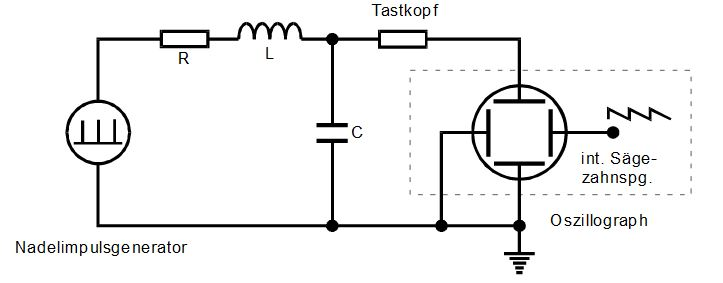
\includegraphics[width=\textwidth]{Bilder/dmpfschalt.JPG}
  \caption{Schaltung für gedämpfte Schwingung}
  \label{fig:schlt1}
\end{figure} \\
Mit Hilfe dieses Aufbaus soll der Abfall der Amplitude eines gedämpften
Schwingkreises untersucht werden. Der Nadelimpulsgenerator wird dabei so
eingestellt, dass die Amplitude der Kondensatorspannung $U_\su{C}$ etwa um
den Faktor 3 bis 8 abnimmt. Die Spannung wird am Oszilloskop gegen die Zeit
aufgetragen.
Abbildung (\ref{fig:dämpfung}) zeigt das ausgegebene Bild des Oszilloskops,
\begin{figure} % Bild kann gerne auch erst in der Auswertung verwendet werden
  \centering
  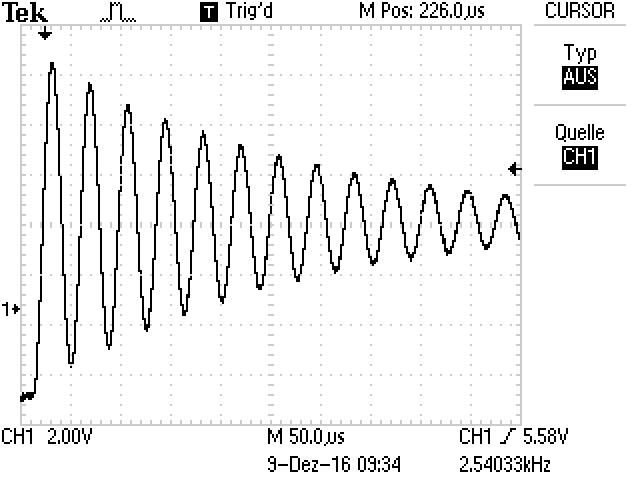
\includegraphics{Bilder/Dmpfung.JPG}
  \caption{Gedämpfte Schwingung am Oszilloskop}
  \label{fig:dämpfung}
\end{figure}
an welchem die Spannungsamplituden mit der zugehörigen Zeitdifferenz $t$
abgelesen werden. Diese Messung ist relativ genau, da der dämpfende Einfluss
des Eingangswiderstands des Oszilloskops mit Hilfe des hochohmigen Tastkopfes
($R_\su{i}=10\,\si{\mega\ohm}$) vernachlässigbar klein gehalten werden.
Zur Messung des Widerstands $R_\su{ap}$ wird die Schaltung aus Abbildung
(\ref{fig:rapschlt}) aufgebaut. \\
\begin{figure}[h]
  \centering
  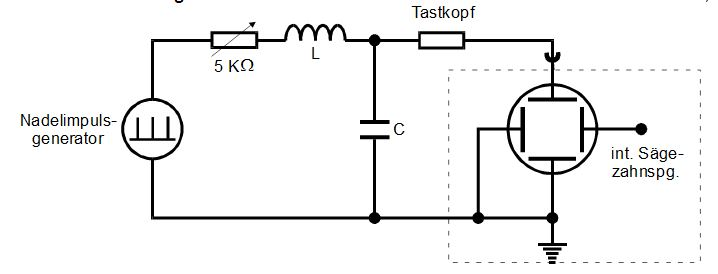
\includegraphics[width=\textwidth]{Bilder/RapSchalt.JPG}
  \caption{Schaltung zur Bestimmung von $R_\su{ap}$}
  \label{fig:rapschlt}
\end{figure}
\newpage
Im Gegensatz zur ersten Messung wird hier ein regulierbarer Widerstand verwendet.
Dieser wird zunächst auf seinen Maximalwert eingestellt, sodass ein Bild
für das Relaxionsverhalten am Oszilloskop angezeigt wird. Dann wird der
Widerstand kontinuierlich verringert, bis ein Überschwingen wie in
Abbildung (\ref{fig:aperid}) zu sehen ist.
\begin{figure}[h]
  \centering
  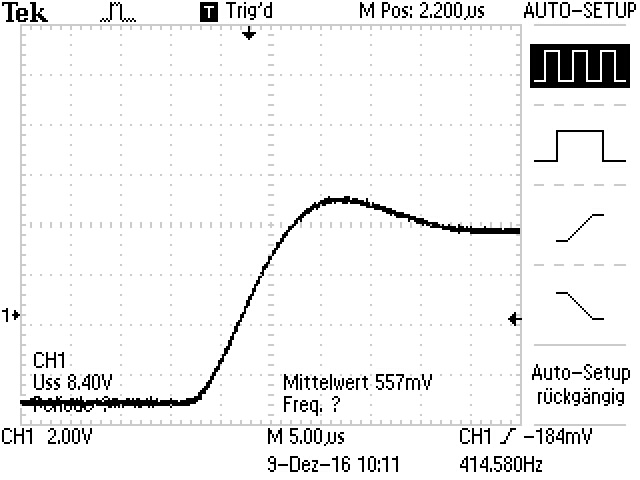
\includegraphics{Bilder/aperid.JPG}
  \caption{Überschwingen der Spannung}
  \label{fig:aperid}
\end{figure} \\
Diesen Zustand bezeichnet man auch als Schwingfall. Der Widerstand soll nun
wieder erhöht werden, bis das Überschwingen gerade verschwindet. Der eingestellte
Widerstand wird als $R_\su{ap}$ notiert.
